\documentclass[14pt,final,titlepage,pscyr]{hedwork}
\usepackage[russian]{babel}
\usepackage[utf8]{inputenc}
\usepackage[derivative]{hedmaths}
\usepackage{graphicx}
\usepackage{array}
\usepackage{listings}
\usepackage{hyperref}
\usepackage{titlesec}
\usepackage{tocloft}

\graphicspath{{images/}}
\renewcommand{\vec}[1]{\mathbf{#1}}

\lstdefinelanguage{OpenCL}{morekeywords=
	{__kernel,kernel,__local,local,__global,global,% 
		__constant,constant,__private,private,% 
		char2,char3,char4,char8,char16,% 
		uchar2,uchar3,uchar4,uchar8,uchar16,% 
		short2,short3,short4,short8,short16,% 
		ushort2,ushort3,ushort4,ushort8,ushort16,% 
		int2,int3,int4,int8,int16,% 
		uint2,uint3,uint4,uint8,uint16,% 
		long2,long3,long4,long8,long16,% 
		ulong2,ulong3,ulong4,ulong8,ulong16,% 
		float2,float3,float4,float8,float16,% 
		image2d_t,image3d_t,sampler_t,event_t,% 
		bool2,bool3,bool4,bool8,bool16,% 
		half2,half3,half4,half8,half16,% 
		quad,quad2,quad3,quad4,quad8,quad16,% 
		complex,imaginary},% 
}% 

\faculty{Факультет электроники и вычислительной техники}
\department{<<Электронно-вычислительные машины и системы>>}
\subject{Вычислительные системы и сетевые технологии}
\topic{Решение системы ОДУ методом Рунге-Кутты 4 порядка}
\variant{9}
\student[m]{студент группы САПР-1.1п\\Голубев~А.~В.}
\teacher[m]{к.т.н. Андреев~А.~Е.}

\titleformat{\section}{\centering\normalsize}{\thesection}{1em}{}
\titlespacing*{\section}{\parindent}{*4}{*4}
\renewcommand{\cfttoctitlefont}{\normalfont\hspace{0.38\textwidth}}
\renewcommand{\cftsecfont}{\hspace{-21pt}}
\renewcommand{\cftparskip}{2mm}
\makeatletter
\renewcommand{\l@section}{\@dottedtocline{1}{0em}{1.25em}}
\makeatother

\begin{document}
\maketitle
\tableofcontents
\newpage
\section{Постановка задач}
\begin{enumerate}
	\item Реализовать с использованием технологий параллельных вычислений задание по вариантам 
		(минимум 2 технологии: MPI и OpenMP, CUDA и OpenMP, OpenMP / OpenCL, Xeon Phi + MPI, 
		MPI / GridGain, cloud computing и т.д.)
	\item Оценить ускорение, степень параллелизма и другие параметры своих реализаций. Построить 
		таблицы и графики на основании тестирования (в зависимости от числа узлов / ядер и от 
		размерности задачи).
	\item Пройти он-лайн тестирование по курсам (\url{www.intuit.ru}): С.А. Немнюгин Основы MPI и 
		Введение в облачные вычисления \\
        \url{http://www.intuit.ru/verifydiplomas/100835677} \\
        \url{http://www.intuit.ru/verifydiplomas/100834994}
\end{enumerate}

\section{Параллельная реализация явного метода Рунге-Кутты}
Метод Рунге -- Кутты позволяет получать одношаговые разностные схемы различного порядка точности, в 
которых в зависимости от точности выбранной формулы правая часть системы может на рассматриваемом шаге 
вычисляется несколько раз.

Для построения вычислительных схем методов Рунге -- Кутты четвёртого порядка в тейлоровском разложении 
искомого решения \( \vec{y}(t) \) учитываются члены, содержащие степени шага \( h = t_{m+1} - t_m \) до 
четвёртой включительно, наиболее часто используемой из которых является следующая:
\begin{equation}
	\vec{y}_{m+1} = \vec{y}_m + \frac{\left( \vec{k}_1 + 2\vec{k}_2 + 2\vec{k}_3 + \vec{k}_4 \right)}{6}
	\label{eq8.9}
\end{equation}
где 
\begin{gather}
	\vec{k}_1 = h\vec{f}\left(t_m, \vec{y}_m \right), \notag \\
	\vec{k}_2 = h\vec{f}\left(t_m + \frac{h}{2}, \vec{y}_m + \frac{\vec{k}_1}{2} \right), \notag \\
	\vec{k}_3 = h\vec{f}\left(t_m + \frac{h}{2}, \vec{y}_m + \frac{\vec{k}_2}{2} \right), \notag \\
	\vec{k}_4 = h\vec{f}\left(t_m + h, \vec{y}_m + \vec{k}_3 \right). \notag
\end{gather}

Схема \eqref{eq8.9} на каждом шаге \( h \) требует четырёх последовательных вычислений правой части 
системы ОДУ для определения значений \( \vec{k}_1, \vec{k}_2, \vec{k}_3, \vec{k}_4 \).

Поскольку в описанной выше вычислительной схеме наиболее трудоёмкой является операции расчёта правых 
частей ОДУ при вычислении \( \vec{k}_i (i = 1, 2, 3, 4) \), то основное внимание следует уделить 
распараллеливанию этой операции. Будем применять поход декомпозиции уравнений системы ОДУ на подсистемы. 
Поэтому для инициализации рассмотрим следующую схему декомпозиции данных по имеющимся процессорным 
элементам с локальной памятью: на каждый \( \mu \)-й ПЭ \( \mu = 0, \ldots, p - 1 ) \) распределяется 
\( n/p \) дифференциальных уравнений и вектор \( \vec{y}_0 \in \mathbb{R}^n \). Далее расчёты 
производятся по следующей схеме:
\begin{enumerate}
	\item на каждой ПЭ одновременно вычисляются \( n/p \) соответствующих компонент вектора 
		\( \vec{k}_1 \) по формуле 
		\[ \left[ \vec{k}_1 \right]_\mu = h\left[ \vec{f}(t_m, \vec{y}_m) \right]_\mu; \]
	\item для обеспечения второго расчётного этапа необходимо провести сборку вектора \( \vec{k}_1 \) 
		целиком на каждом ПЭ. Затем независимо выполняется вычисление компонент вектора \( \vec{k}_2 \) 
		по формуле 
	\[ 
		\left[ \vec{k}_2 \right]_\mu = 
			h\left[ 
			\vec{f}(t_m + \frac{h}{2}, \vec{y}_m + \frac{\vec{k}_1}{2}) 
			\right]_\mu; 
	\]
    \item проводится сборка вектора \( \vec{k}_2 \) на каждом ПЭ, вычисляются компоненты вектора 
    	\( \vec{k}_3 \): 
		\[ 
			\left[ \vec{k}_3 \right]_\mu = 
			h\left[ 
				\vec{f}(t_m + \frac{h}{2}, \vec{y}_m + \frac{\vec{k}_2}{2}) 
			\right]_\mu; 
		\]
	\item проводится сборка вектора \( \vec{k}_3 \) на каждом ПЭ, вычисляются компоненты вектора 
		\( \vec{k}_4 \):
		\[ \left[ \vec{k}_4 \right]_\mu = h\left[ \vec{f}(t_m, \vec{y}_m + \vec{k}_3 ) \right]_\mu; \]
		\item рассчитываются с идеальным параллелизмом компоненты вектора \( \vec{y}_{m+1} \) : 
		\[
			\left[ \vec{y}_{m+1} \right]_\mu = \left[ \vec{y}_m \right]_\mu + \frac{1}{6}\left( 
				\left[ \vec{k}_1 \right]_\mu + 2\left[ \vec{k}_2 \right]_\mu + 
				2\left[ \vec{k}_3 \right]_\mu + \left[ \vec{k}_4 \right]_\mu
			\right)
		\]
		и производится сборка вектора \( \vec{y}_{m+1} \) на каждом ПЭ. Если необходимо продолжить 
		вычислительный процесс, то полагается \( m = m + 1 \) и осуществляется переход на пункт 1.
\end{enumerate}

Заметим, что в данном алгоритме производится четыре операции вычисления вектора правых частей ОДУ, 
шестнадцать операций сложения векторов и умножения вектора на число и четыре операции глобальной 
сборки векторов. 

В случае, когда \( \vec{f}(t, \vec{y}(t)) \equiv A \times \vec{y}(t) \), где 
\( A \in \mathbb{R}^{n\times n} \) -- матрица с постоянными коэффициентами, можно получить алгоритм, 
который имеет меньшее число межпроцессорных пересылок данных на одной итерации метода Рунге -- Кутты. 
Для этого построим оператор перехода для одного вычислительного шага, позволяющий определить 
значение вектора неизвестных на следующей итерации \( \vec{y}_{m+1} \) через \( \vec{y}_m \). 
Преобразуем значения \( \vec{k}_1, \vec{k}_2, \vec{k}_3, \vec{k}_4 \):
\begin{gather}
	\vec{k}_1 = hA\vec{y}_m, \notag \\
	\vec{k}_2 = hA\left(\vec{y}_m + \frac{\vec{k}_1}{2}\right) = 
		\vec{k}_1 + \left(\frac{h}{2}\right)A\vec{k}_1 = 
		\left( E + \left(\frac{h}{2}\right)A \right)\vec{k}_1 = 
		h\left( E + \left(\frac{h}{2}A \right)A \right) \vec{y}_m, \notag \\
	\vec{k}_3 = hA\left( \vec{y}_m + \frac{1}{2}\vec{k}_2 \right) = 
		\vec{k}_1 + \left( \frac{h}{2} \right)A\vec{k}_2 = 
		\vec{k}_1 + \left( \frac{h}{2} \right)A\left( \vec{k}_1 + 
		\left( \frac{h}{2} \right)A\vec{k}_1 \right) = \notag \\ =
		h\left( E + \left( \frac{h}{2} \right)A + \left( \frac{h}{2} \right)^2 A^2 \right)A\vec{y}_m, 
	\notag \\
	\vec{k}_4 = hA\left( \vec{y}_m + \vec{k}_3 \right) = 
		\vec{k}_1 + \left( hA + \left( \frac{h^2}{2} \right)A^2 + 
			\left( \frac{h^3}{4} \right)A^3 \right)\vec{k}_1 = \notag \\ = 
		h\left( E + hA + \left( \frac{h^2}{2} \right)A^2 + 
			\left( \frac{h^3}{4} \right)A^3 \right)A\vec{y}_m
	\notag
\end{gather}
и, подставив из в \eqref{eq8.9}, получим
\begin{gather}
	\vec{y}_{m+1} = B\vec{y}_m; \quad
	B = E + hA\left( E + \left( \frac{h}{2} \right)A\left( 
		E + \left( \frac{h}{3} \right) A \left( E + \left( \frac{h}{4} \right)A \right) 
	\right) \right)
	\label{eq8.10}
\end{gather}
где \( B \) -- оператор перехода.

Рассчитав заранее матрицу \( B \), получим вычислительный алгоритм, в котором каждое новое значение 
вектора \( \vec{y}_{m+1} \) определяется за один шаг умножения матрицы \( B \) на вектор.

При параллельной реализации \eqref{eq8.10} умножение блочных строк матрицы \( B \) на вектора 
\( \vec{y}_m \) будет проводиться одновременно и независимо. Потребуется только после каждого 
вычислительного шага по \eqref{eq8.10} проводить сборку вектора \( \vec{y}_{m+1} \) на всех процессорных 
элементах.\cite{methods}

\section{Используемый пример}
В качестве примера используем СОДУ для расчёта направления силовых линий для различных векторных 
полей. Систему уравнений можно записать следующим образом:

\[
	\vec{A}(\vec{0}) = \vec{r}_0, \quad \cfrac{d\vec{r}}{dt} = \vec{A}\left( \vec{r}(t) \right)
\]

где \( \vec{A}(\vec{r}) \) -- векторное поле, \( \vec{r}(t) \) -- интегральная кривая, 
\( \vec{r}_0 \) -- начальное условие.

\newpage

\section{Используемое оборудование}
\noindentТестирование программ производилось на следующем оборудовании:
\begin{table}[h]
    \center
    \begin{tabular}{|C{5cm}|C{2cm}|C{2cm}|C{3cm}|C{3cm}|}
        \hline
        Оборудование & Частота, Ггц & Кол-во ядер, шт & float, GFLOPS/s & double, GFLOPS/s \\ \hline
        AMD Opteron(TM) Processor 6272 & 2.10 & 64 & - & - \\ \hline
        Intel(R) Core(TM) i5-4690 & 3.5 & 4 & 3.7 & 3.7 \\ \hline
        GIGABYTE Radeon R9 280X & 1.10 & 32 & 4400 & 1112 \\ \hline
    \end{tabular}
\end{table}

\noindentИспользуемые операционные системы:
\begin{enumerate}
	\item CentOS release 6.5 (Final) / Linux version 2.6.32-431.el6.x86\_64
	\item Arch Linux / Linux 3.17.6-1-ARCH x86\_64
\end{enumerate}

\noindentИспользуемые версии компиляторов:
\begin{enumerate}
	\item gcc version 4.4.7 20120313 (Red Hat 4.4.7-11) (GCC)
	\item gcc version 4.9.2 20141224 (prerelease) (GCC) 
\end{enumerate}

\noindentФлаги оптимизации скомпилированных программ:
\begin{enumerate}
	\item -O3 -m64 -march=bdver1 -mavx -msse -msse2 -msse3 -msse4 -msse4.1 \\
		-msse4.2 -msse4a -mssse3 -mfpmath=387,sse -pipe
	\item -O3 -m64 -march=haswell -mavx -mavx2 -mmmx -mmovbe -msse \\
		-msse2 -msse3 -msse4 -msse4.1 -msse4.2 -mssse3 -mfpmath=sse,387 \\
		-ffast-math -flto -pipe
\end{enumerate}

\newpage

\section{Последовательная программа}
Параллельная и последовательная программа реализованы в качестве заменяемого ядра. Исходный код ядер для 
последовательной (default) и параллельных (OpenMP, OpenCL) программ представлены в разделе 
Приложение \eqref{sec:app}.

Результаты проведенных тестов представлены в разделе \ref{sec:test}. 

\section{Оценка алгоритма}
Время последовательного алгоритма для одного уравнения при реализации метода Рунге -- Кутта может быть 
описано следующим соотношением:
\[
	T_1 = s\cdot T_f + N \cdot \left[ s^2 \cdot t_\text{умн} + s^2 \cdot t_\text{сл} + 
		s \cdot T_f \right] + s \cdot t_\text{умн} + s \cdot t_\text{сл}
\]
где \( T_f \) -- время вычисления функции \( f \) -- правой части исходного дифференциального уравнения;
\( t_\text{умн} \) -- время выполнения операции одиночного умножения; \( t_\text{сл} \) -- время 
выполнения операции одиночного сложения; \( N \) -- число итераций в методе. Для представленного алгоритма 
время выполнения на \( p \) процессорах без учёта обменов и других накладных расходов задаётся соотношением:
\[
	T_p = T_f + N \cdot \left[ s \cdot t_\text{умн} + s \cdot t_\text{сл} + T_f \right] + 
		t_\text{умн} + t_\text{сл}
\]

Соответственно, коэффициент ускорения равен
\[
	S_p = \frac{T_1}{T_p} = \frac{s\cdot T_f + N\cdot\left[ 2s^2 \cdot t* + s\cdot T_f\right] + 2s\cdot t*}
			{T_f + N\cdot\left[ 2s\cdot t* + T_f\right] + 2\cdot t*}
\]
При подсчёте коэффициента ускорения будем считать, что \( t_\text{сл} = t_\text{умн} = t* \) -- любая 
арифметическая операция с плавающей точкой выполняется за одно и то же время независимо от вида операции.
Коэффициент ускорения для сложных функций правой части коэффициент ускорения практически равен числу 
процессоров:
\[
	S_p \approx \frac{s \cdot T_f + N \cdot s \cdot T_f}{T_f + N \cdot T_f } = s = p
\]

Тогда показатель эффективности будет равен:
\[
	E_p = \frac{T_1(n)}{pT_p(n)} = \frac{1}{p}S_p(n) = 1
\]

\newpage

Получим значение достижимого ускорения, при учёте, что \( f = 3/10 \):
\[
    S_p = \frac{1}{f + (1-f)/p} = \frac{1}{\cfrac{3}{10} + \cfrac{7}{10} \cdot \cfrac{1}{p}}
\]
где \( f \) -- доля последовательных вычислений, \( p \) -- количество процессоров.

Тогда показатель эффективности можно записать, как:
\[
    E_p = \frac{1}{p}\frac{1}{f + (1-f)/p} = \frac{1}{\cfrac{3}{10}\cdot p + \cfrac{7}{10}}
\]

\begin{figure}[ht!]
    \center
    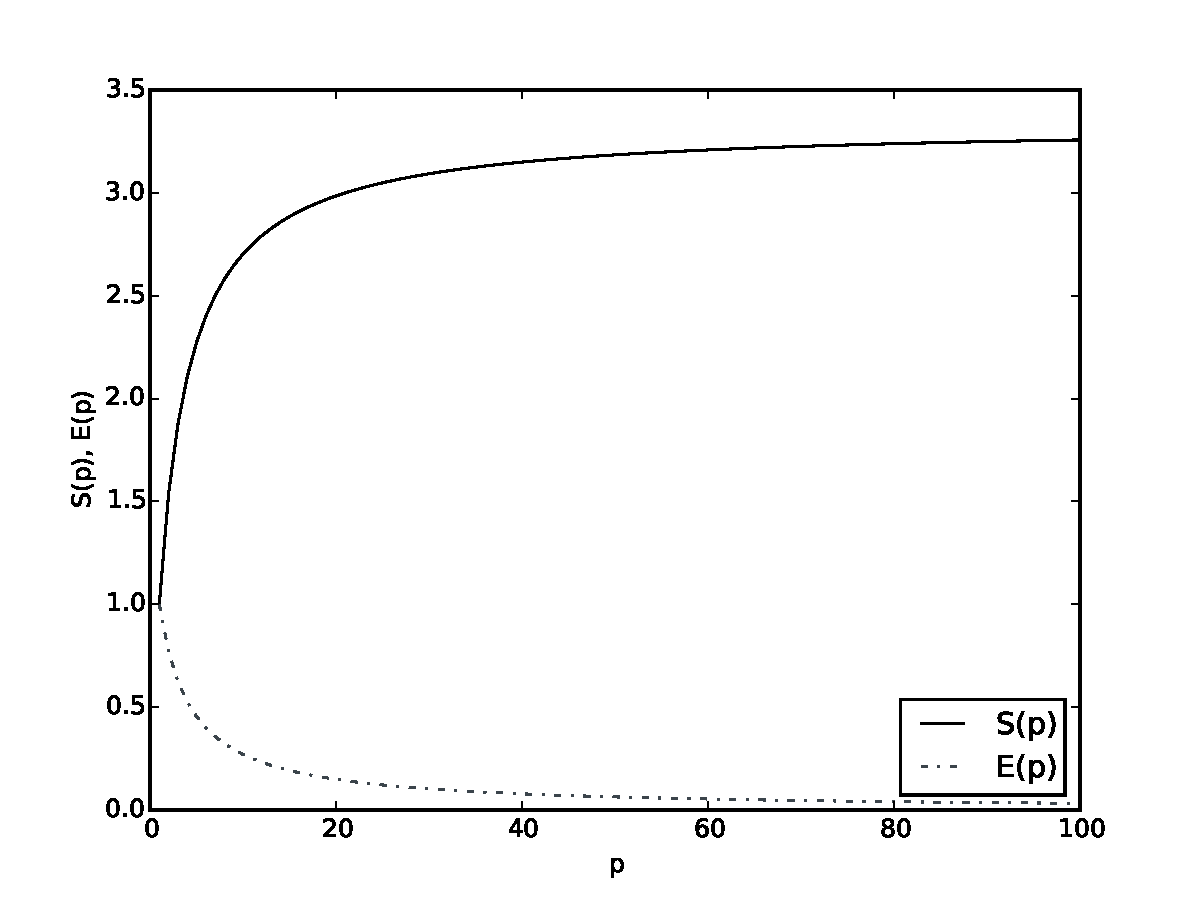
\includegraphics[width=0.8\textwidth]{amhdal_eff}
    \caption{Достижимое ускорение по закону Амдаля \( S(p) \) и показатель эффективности \( E(p) \)}
\end{figure}

\newpage

\section{Входные данные}
Тестирование последовательной и параллельной программы производилось на следующем наборе данных
\begin{table}[h]
    \center
	\begin{tabular}{|c|c|c|c|c|c|c|c|c|}
		\hline
		Шаг & \multicolumn{8}{c|}{Количество точек} \\ \hline
		\( 10^{-8} \) & 100 & 1000 & 5000 & 10000 & 50000 & 100000 & 150000 & 200000 \\ 
		\hline
	\end{tabular}
\end{table}

Программы для генерации входных данных доступны в конце приложения.

\newpage

\section{Результаты}
\label{sec:test}
Результаты полученные на кластере:
\begin{figure}[ht!]
    \begin{minipage}{0.55\textwidth}
        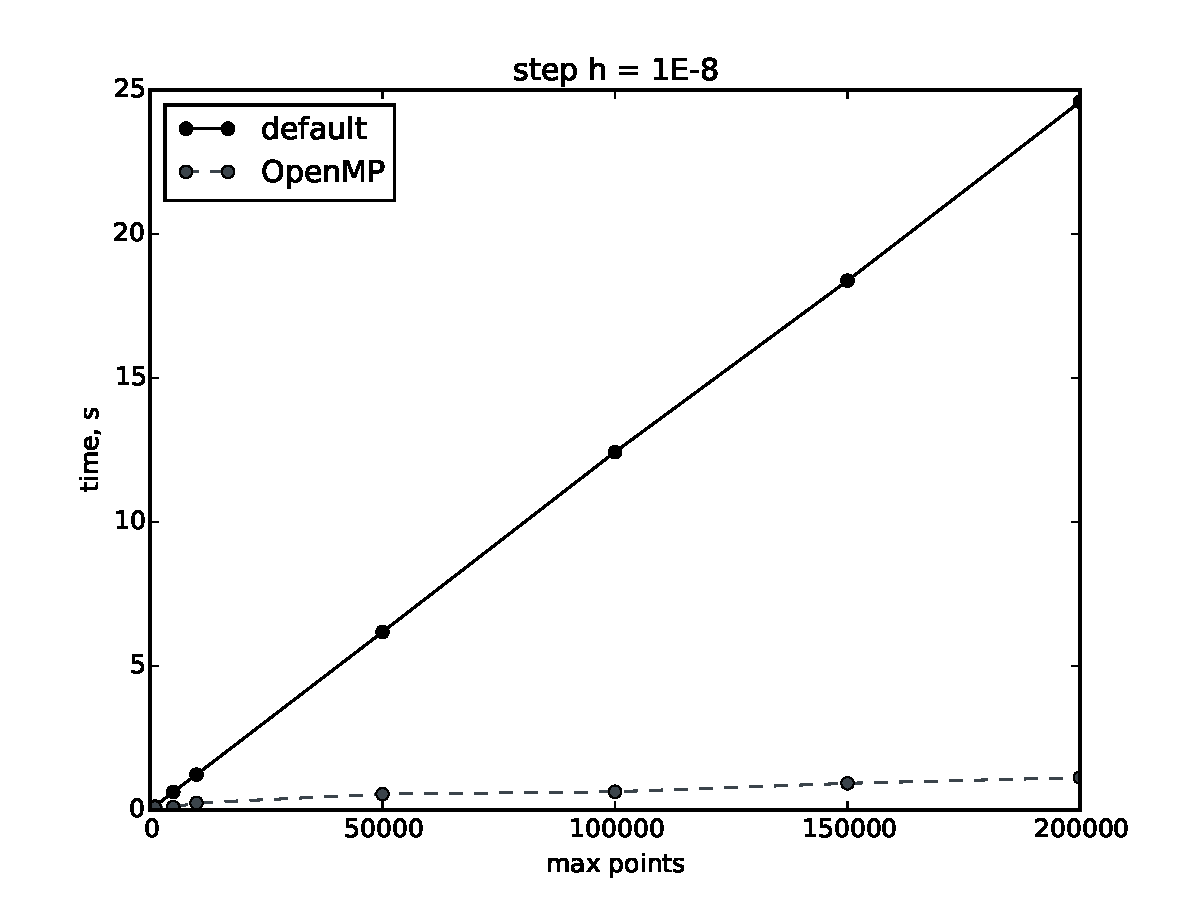
\includegraphics[width=\textwidth]{linesField_cl_1E-8}
    \end{minipage}
    \begin{minipage}{0.47\textwidth}
        \begin{tabular}{|c|c|c|}
            \hline
            Шаг & default, с & OpenMP, с \\ \hline
            1.00\cdot10^{2} & 1.00\cdot10^{-2} & 7.41\cdot10^{-2} \\ \hline
            1.00\cdot10^{3} & 1.20\cdot10^{-1} & 8.64\cdot10^{-2} \\ \hline
            5.00\cdot10^{3} & 6.30\cdot10^{-1} & 9.62\cdot10^{-2} \\ \hline
            1.00\cdot10^{4} & 1.23 & 2.45\cdot10^{-1} \\ \hline
            5.00\cdot10^{4} & 6.18& 5.52\cdot10^{-1} \\ \hline
            1.00\cdot10^{5} & 1.24\cdot10^{1} & 6.35\cdot10^{-1} \\ \hline
            1.50\cdot10^{5} & 1.84\cdot10^{1} & 9.27\cdot10^{-1} \\ \hline
            2.00\cdot10^{5} & 2.46\cdot10^{1} & 1.13 \\ \hline
        \end{tabular}
    \end{minipage}
    \caption{linesField (256 потоков)}
\end{figure}

\begin{figure}[ht!]
    \begin{minipage}{0.55\textwidth}
        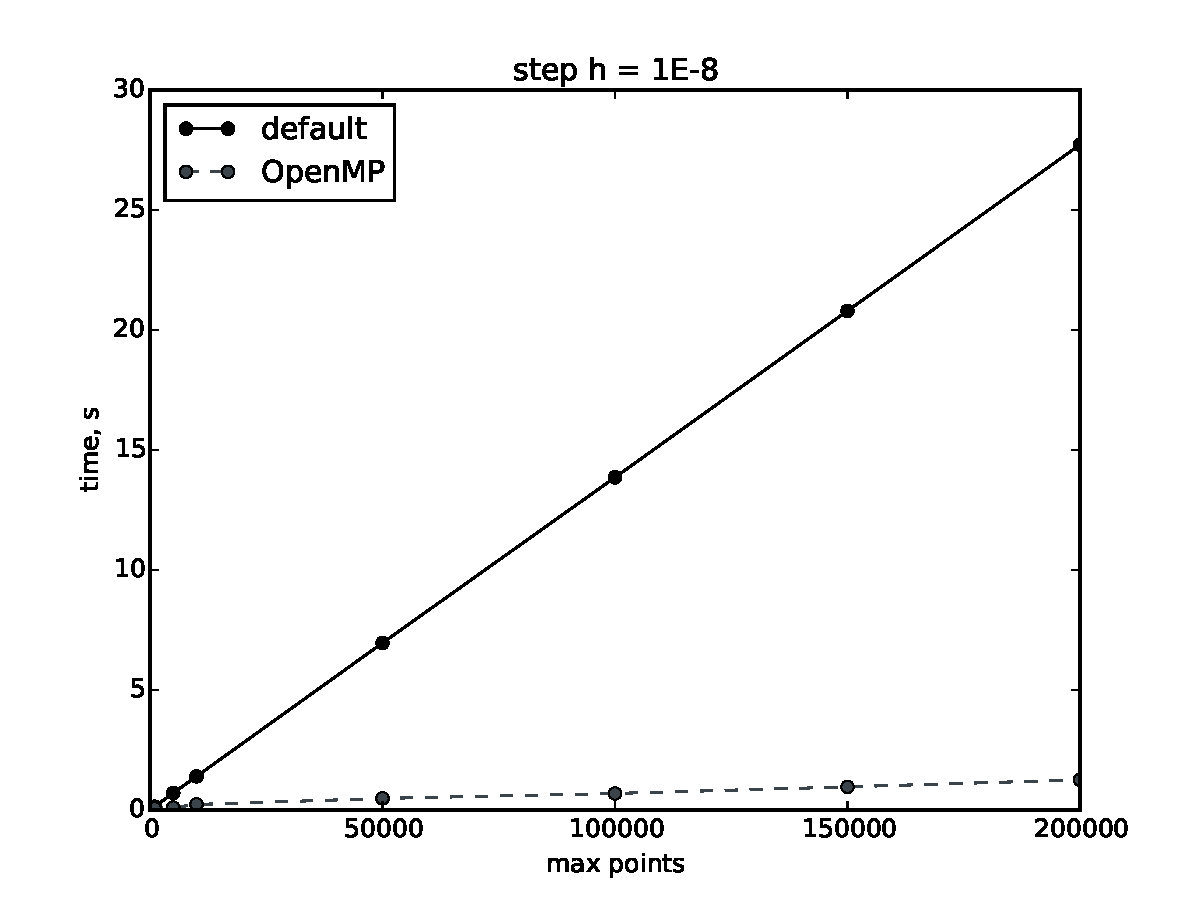
\includegraphics[width=\textwidth]{randomField_cl_1E-8}
    \end{minipage}
    \begin{minipage}{0.47\textwidth}
        \begin{tabular}{|c|c|c|}
            \hline
            Шаг & default, с & OpenMP, с \\ \hline
            1.00\cdot10^{2} & 1.00\cdot10^{-2} & 7.59\cdot10^{-2} \\ \hline
            1.00\cdot10^{3} & 1.40\cdot10^{-1} & 6.79\cdot10^{-2} \\ \hline
            5.00\cdot10^{3} & 7.10\cdot10^{-1} & 1.02\cdot10^{-1} \\ \hline
            1.00\cdot10^{4} & 1.40 & 2.31\cdot10^{-1} \\ \hline
            5.00\cdot10^{4} & 6.96 & 4.82\cdot10^{-1} \\ \hline
            1.00\cdot10^{5} & 1.39\cdot10^{1} & 6.90\cdot10^{-1} \\ \hline
            1.50\cdot10^{5} & 2.08\cdot10^{1} & 9.65\cdot10^{-1} \\ \hline
            2.00\cdot10^{5} & 2.77\cdot10^{1} & 1.26 \\ \hline
        \end{tabular}
    \end{minipage}
    \caption{randomField (256 потоков)}
\end{figure}

\newpage

\begin{figure}[ht!]
    \begin{minipage}{0.55\textwidth}
        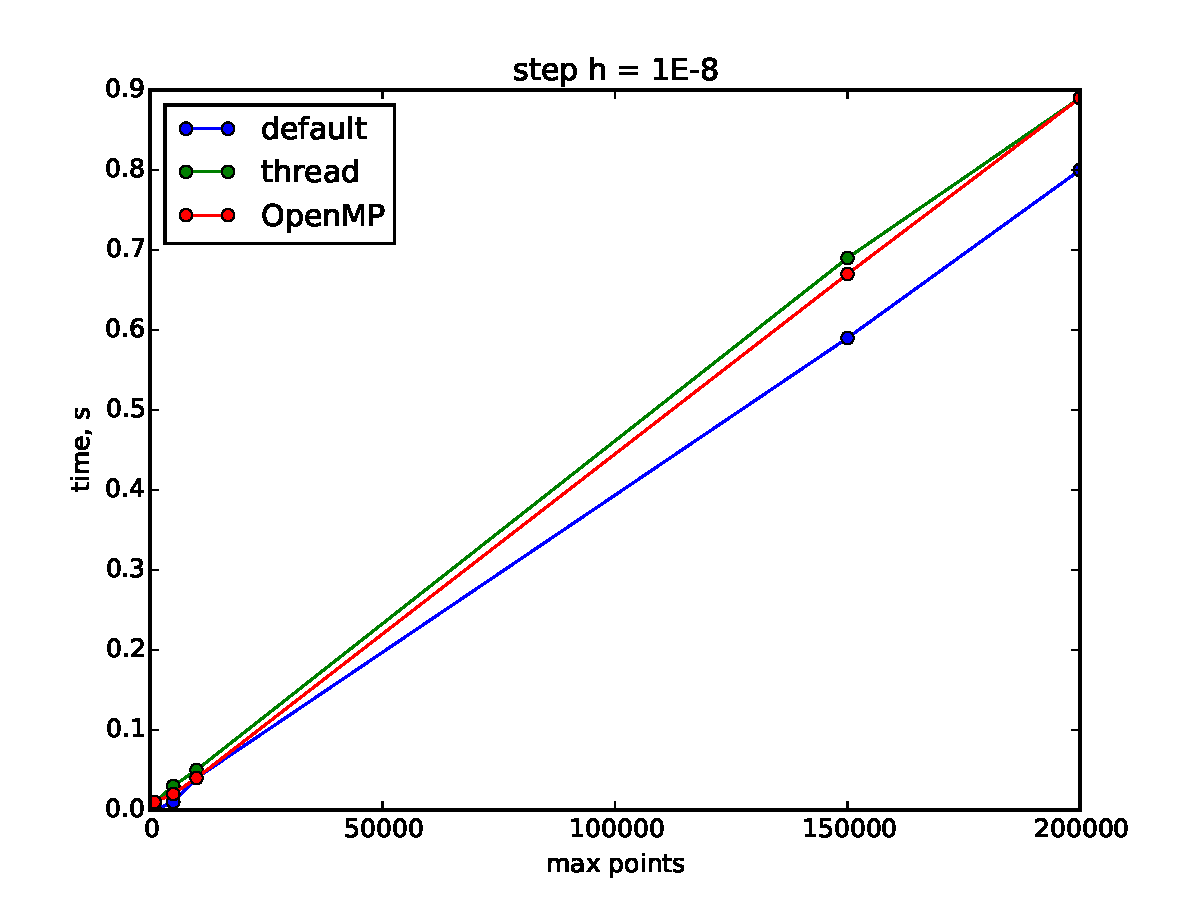
\includegraphics[width=\textwidth]{rotationField_cl_1E-8}
    \end{minipage}
    \begin{minipage}{0.47\textwidth}
        \begin{tabular}{|c|c|c|}
            \hline
            Шаг & default, с & OpenMP, с \\ \hline
            1.00\cdot10^{2} & 0.00 & 1.17\cdot10^{-3} \\ \hline
            1.00\cdot10^{3} & 0.00 & 1.63\cdot10^{-3} \\ \hline
            5.00\cdot10^{3} & 2.00\cdot10^{-2} & 3.75\cdot10^{-3} \\ \hline
            1.00\cdot10^{4} & 5.00\cdot10^{-2} & 6.75\cdot10^{-3} \\ \hline
            5.00\cdot10^{4} & 2.10\cdot10^{-1} & 2.93\cdot10^{-2} \\ \hline
            1.00\cdot10^{5} & 4.00\cdot10^{-1} & 5.90\cdot10^{-2} \\ \hline
            1.50\cdot10^{5} & 6.10\cdot10^{-1} & 8.72\cdot10^{-2} \\ \hline
            2.00\cdot10^{5} & 8.00\cdot10^{-1} & 1.14\cdot10^{-1} \\ \hline
        \end{tabular}
    \end{minipage}
    \caption{rotationField (7 потоков)}
\end{figure}

\newpage

Результаты полученные на стационарном компьютере:
\begin{table}[ht!]
    \center
    \begin{tabular}{|c|c|c|c|}
        \hline
        Шаг & default, с & OpenMP, с & OpenCL, с \\ \hline
        1.00\cdot10^{2} & 3.12\cdot10^{-3} & 3.73\cdot10^{-3} & 1.28\cdot10^{-3} \\ \hline
        1.00\cdot10^{3} & 3.09\cdot10^{-2} & 1.67\cdot10^{-2} & 1.21\cdot10^{-2} \\ \hline
        5.00\cdot10^{3} & 1.54\cdot10^{-1} & 7.89\cdot10^{-2} & 6.08\cdot10^{-2} \\ \hline
        1.00\cdot10^{4} & 3.08\cdot10^{-1} & 2.40\cdot10^{-1} & 1.22\cdot10^{-1} \\ \hline
        5.00\cdot10^{4} & 1.54 & 5.61\cdot10^{-1} & 6.13\cdot10^{-1} \\ \hline
        1.00\cdot10^{5} & 3.07 & 9.10\cdot10^{-1} & 1.23 \\ \hline
        1.50\cdot10^{5} & 4.59 & 1.34 & 1.85 \\ \hline
        2.00\cdot10^{5} & 6.12 & 1.71 & 2.46 \\ \hline
    \end{tabular}
\end{table}

\begin{figure}[ht!]
    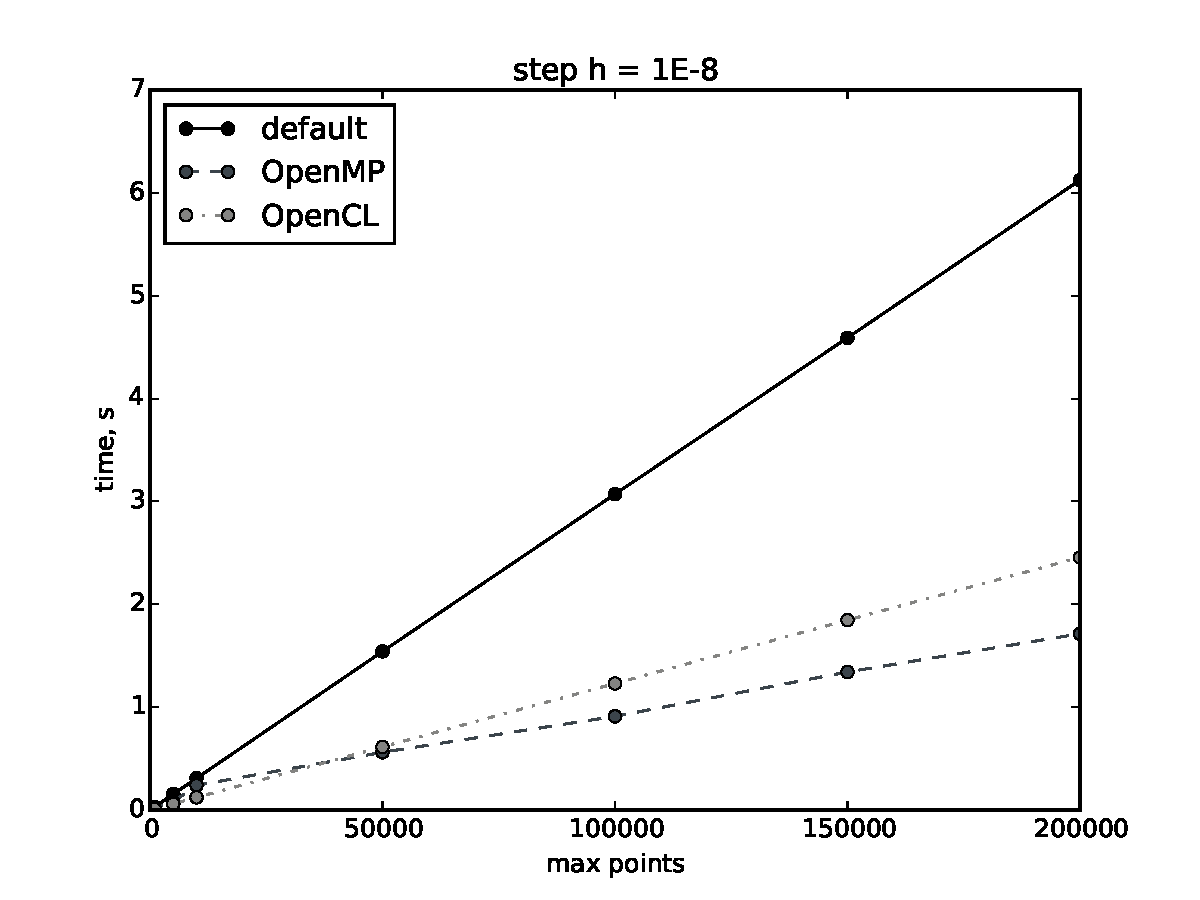
\includegraphics[width=\textwidth]{linesField_my_1E-8}
    \caption{linesField (256 потоков)}
    \label{img:line}
\end{figure}

\newpage

\begin{table}[ht!]
    \center
    \begin{tabular}{|c|c|c|c|}
        \hline
        Шаг & default, с & OpenMP, с & OpenCL, с \\ \hline
        1.00\cdot10^{2} & 3.16\cdot10^{-3} & 4.09\cdot10^{-3} & 1.70\cdot10^{-3} \\ \hline
        1.00\cdot10^{3} & 3.09\cdot10^{-2} & 1.88\cdot10^{-2} & 1.66\cdot10^{-2} \\ \hline
        5.00\cdot10^{3} & 1.54\cdot10^{-1} & 1.18\cdot10^{-1} & 8.33\cdot10^{-2} \\ \hline
        1.00\cdot10^{4} & 3.09\cdot10^{-1} & 1.87\cdot10^{-1} & 1.62\cdot10^{-1} \\ \hline
        5.00\cdot10^{4} & 1.54 & 6.11\cdot10^{-1} & 8.16\cdot10^{-1} \\ \hline
        1.00\cdot10^{5} & 3.07 & 9.34\cdot10^{-1} & 1.62\\ \hline
        1.50\cdot10^{5} & 4.59 & 1.31 & 2.52 \\ \hline
        2.00\cdot10^{5} & 6.13 & 1.69 & 3.48 \\ \hline
    \end{tabular}
\end{table}

\begin{figure}[ht!]
    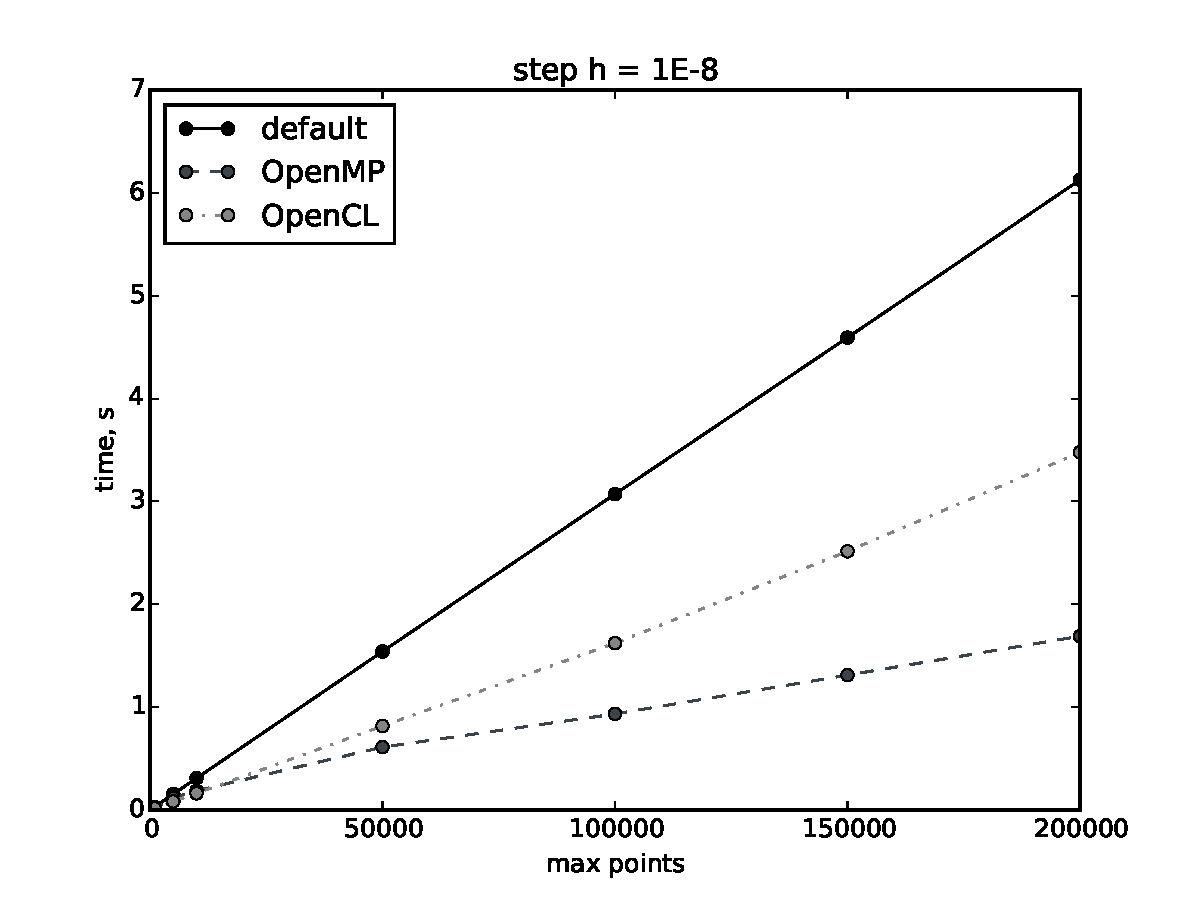
\includegraphics[width=\textwidth]{randomField_my_1E-8}
    \caption{randomField (256 потоков)}
    \label{img:rand}
\end{figure}

\newpage

\begin{table}[ht!]
    \center
    \begin{tabular}{|c|c|c|c|}
        \hline
        Шаг & default, с & OpenMP, с & OpenCL, с \\ \hline
        1.00\cdot10^{2} & 9.70\cdot10^{-5} & 3.58\cdot10^{-4} & 3.22\cdot10^{-3} \\ \hline
        1.00\cdot10^{3} & 9.45\cdot10^{-4} & 6.20\cdot10^{-4} & 2.39\cdot10^{-2} \\ \hline
        5.00\cdot10^{3} & 4.66\cdot10^{-3} & 2.04\cdot10^{-3} & 7.10\cdot10^{-2} \\ \hline
        1.00\cdot10^{4} & 9.37\cdot10^{-3} & 3.81\cdot10^{-3} & 1.42\cdot10^{-1} \\ \hline
        5.00\cdot10^{4} & 4.67\cdot10^{-2} & 1.74\cdot10^{-2} & 7.08\cdot10^{-1} \\ \hline
        1.00\cdot10^{5} & 9.34\cdot10^{-2} & 2.62\cdot10^{-2} & 1.42 \\ \hline
        1.50\cdot10^{5} & 1.39\cdot10^{-1} & 4.54\cdot10^{-2} & 2.13 \\ \hline
        2.00\cdot10^{5} & 1.85\cdot10^{-1} & 5.54\cdot10^{-2} & 2.84 \\ \hline
    \end{tabular}
\end{table}

\begin{figure}[ht!]
    \center
    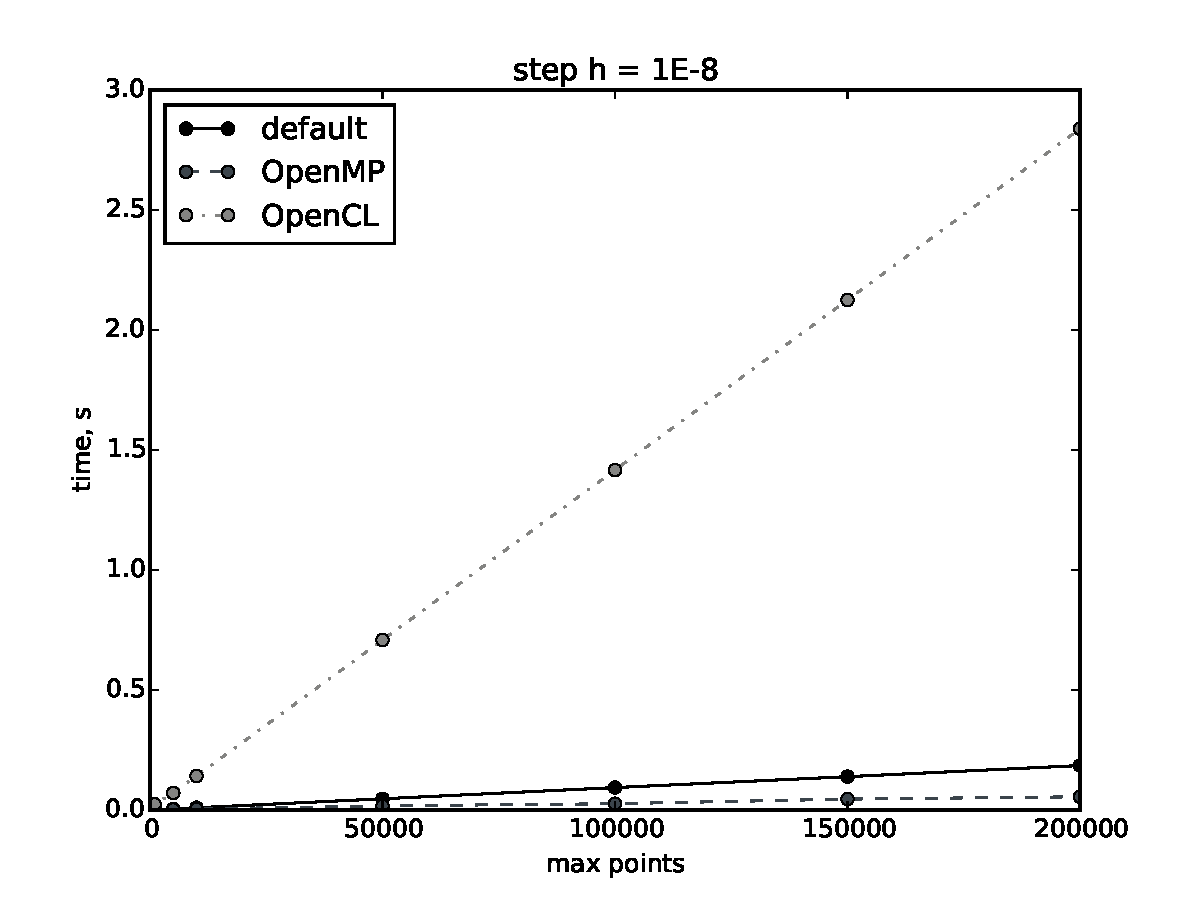
\includegraphics[width=\textwidth]{rotationField_my_1E-8}
    \caption{rotationField (8 потоков)}
    \label{img:rot}
\end{figure}

\newpage

\section{Выводы}
В ходе семестровой работы был рассмотрен и реализован параллельный метод Рунге -- Кутты для системы ОДУ, 
написаны программы для последовательной (default) и параллельных (OpenMP, OpenCL) версий. 

Произведена теоретическая оценка коэффициента ускорения и показателя эффективности. Проведены практические 
работы по замеру времени выполнения алгоритма при разных входных данных на разном оборудовании. 

При малом количестве точек в системе выигрыш по скорости параллельной программы незначительный, но при их 
увеличении разрыв становиться значительным. Так же важной особенностью является размерность задачи, так 
как при малых значениях эффективность расчёта с использованием OpenCL резко снижается (рис.~\ref{img:rot}).

На рисунках \ref{img:line} и \ref{img:rand} отставание программы с использованием OpenCL от программы на 
OpenMP, которое можно объяснить временем затраченным на передачу и сбор данных.

\newpage

\renewcommand{\bibname}{Список используемой литературы}
\addcontentsline{toc}{section}{Список используемой литературы}
\begin{thebibliography}{10}
	\bibitem{methods} Cтарченко, А.~В. Методы параллельных вычислений~/ А.~В. Старченко, В.~Н. Берцун ~// 
		Томский государственный университет "--- 2013
	\bibitem{theory} Назарова, И.~А. Параллельные полностью неявные методы численного решения жестких 
		задач для СОДУ~/ И.~А. Назарова ~// Донецкий национальный технический университет "--- 2005
	\bibitem{book01} Горелов, Ю.~Н. Численные методы решений обыкновенных дифференциальных уравнений 
		(метод Рунге -- Кутта) ~/ Ю.~Н. Горелов ~// Самарский университет "--- 2006
	\bibitem{book02} Баркалов, К.~А. Образовательный комплекс <<Параллельные численные методы>> ~/ 
		К.~А. Баркалов ~// Нижний Новгород "--- 2011
	\bibitem{book03} Clauß, M. Simulating the Spread of Epidemics in Real-world Trading Networks 
		using OpenCL ~/ Martin Clauß "--- 10.02.2012
\end{thebibliography}

\newpage

\addcontentsline{toc}{section}{Приложение}
\label{sec:app}
\centerОбщая часть для всех программ:
\lstinputlisting[language=C++, basicstyle=\tiny, firstline=1, lastline=100]{code/rk_kernel_default.cpp}

\newpage

Ядро последовательной программы:
\lstinputlisting[language=C++, basicstyle=\tiny, firstline=100]{code/rk_kernel_default.cpp}

\newpage

Ядро программы использующая OpenMP:
\lstinputlisting[language=C++, basicstyle=\tiny]{code/rk_kernel_openmp.cpp}

\newpage

Ядро программы использующая OpenCL:
\lstinputlisting[language=OpenCL, basicstyle=\tiny]{code/rk_kernel_opencl.cl}

Настройка и работа с OpenCL:
\lstinputlisting[language=C++, basicstyle=\tiny]{code/opencl_init.cpp}

Структуры данных:
\lstinputlisting[language=C++, basicstyle=\tiny]{code/args.h}
\lstinputlisting[language=C++, basicstyle=\tiny]{code/dataset.cpp}
\lstinputlisting[language=C++, basicstyle=\tiny]{code/fiber.cpp}

Программы генерации входных данных:
\lstinputlisting[language=C, basicstyle=\tiny]{code/lines.c}
\lstinputlisting[language=C, basicstyle=\tiny]{code/random.c}
\lstinputlisting[language=C, basicstyle=\tiny]{code/rotation.c}

\end{document}
